\pdfminorversion=4
\pdfobjcompresslevel=0
%% FinReason Cup 2026 -- Task 1 Working Notes (challenge paper)
%% IEEE two-column conference format (IEEEtran), single-blind (authors shown).
%% Build:  pdflatex main && bibtex main && pdflatex main && pdflatex main
\documentclass[conference]{IEEEtran}

\usepackage{cite}
\usepackage{amsmath,amssymb}
\usepackage{graphicx}
\usepackage{array}
\usepackage{textcomp}
\usepackage{tikz}
\usetikzlibrary{arrows.meta,positioning}
\usepackage{url}

\hyphenation{FinReason Fin-Chain template-specific pre-defined}

\begin{document}

\title{Learning Verifiable Financial Formulas from Templates:\\
Hybrid Symbolic Solving for FinReason Cup 2026, Task~1}

% ---- Single-blind review: keep names and affiliations ----
\author{\IEEEauthorblockN{Umar Tabbsum}
\IEEEauthorblockA{Team \texttt{ut1776}}}

\maketitle

\begin{abstract}
Task~1 of the FinReason Cup at IEEE Big Data 2026 asks systems to solve
templated financial problems and to report a typed final answer and the values
of published intermediate reasoning steps. We describe a hybrid symbolic system.
A library of hand-written exact solvers covers only 17 of 290 published
templates. Our main contribution is a generic formula learner: for each template
it searches a small arithmetic grammar for expressions that reproduce the
labeled final answers and every intermediate step, and it reuses learned steps
as building blocks for later expressions. Accepted programs are checked with
exact rational arithmetic. This establishes agreement with the labeled examples
under the scoring rules, not correctness on new instances, and the system
abstains otherwise. Scored with the organizers' scorer on held-out instances of
seen templates, the learner answers 191 of 290 questions correctly
(final-answer score 0.659 against 0.059 for the hand-written library) and
matches 332 of 518 reasoning steps, with 99.5\% precision on the questions it
answers. An ablation at a fixed search budget shows that step reuse is
essential: forbidding final-answer expressions from using learned steps cuts
correct answers from 191 to 75. In the official final results the system
answered 406 of 928 test questions and 377 correctly, a combined final-answer
score of 0.336 (rank 27 of 27). The score on templates with released examples,
about 0.62, is close to our held-out estimate, whereas the hidden-template
stratum scores 0.055. We analyze the remaining failures and outline next steps.
\end{abstract}

\begin{IEEEkeywords}
financial reasoning, programming by example, formula learning, exact
arithmetic, verifiable reasoning, symbolic benchmarks
\end{IEEEkeywords}

% =====================================================================
\section{Introduction}
Financial question answering is unforgiving: an answer that is off by a
rounding convention is simply wrong. Task~1 of the FinReason Cup asks
participants to solve multi-step financial problems and to return a typed final
answer together with values for published intermediate reasoning
steps~\cite{finreason2026overview,finreason2026task1overview}. The questions are
generated from symbolic templates, following the FinChain
benchmark~\cite{xie-etal-2026-finchain}, so every question has a single
verifiable ground truth and a fixed reasoning trace. This setting differs from
open-ended financial question answering over reports~\cite{chen-etal-2021-finqa}
in one respect that matters for system design: the answer is a deterministic
function of the numbers in the question, and the function depends only on the
template.

Our entry began as the obvious engineering response to this structure: write an
exact solver for each template. That approach is accurate but slow. After
several iterations our hand-written library solved 17 of 290 templates. The
more interesting observation is that the organizers also release ten or more
labeled instances of every template, and a labeled instance is exactly a
programming-by-example specification~\cite{gulwani2017program}. We therefore
replaced the per-template engineering with a generic learner that recovers each
template's formulas from its examples. The learner is conservative: it returns a
formula only if the formula reproduces every labeled example exactly, and it
abstains otherwise.

\textbf{Contributions.}
\begin{itemize}
  \item A \emph{template formula learner} that combines enumerative search with
        value-signature pruning, meet-in-the-middle matching, rounding-aware
        comparison, and chained intermediate steps, and verifies every
        accepted program with exact rational arithmetic (Section~\ref{sec_method}).
  \item An evaluation with the organizers' official scorer on held-out
        instances, with ablations, a learning curve, and a failure taxonomy
        (Sections~\ref{sec_protocol} and~\ref{sec_results}).
  \item A quantitative account of template reuse across splits, showing how
        much of the test set a template-level method can reach.
  \item A prioritized, evidence-based list of improvements
        (Section~\ref{sec_future}) and the data behind every figure and table.
\end{itemize}

% =====================================================================
\section{Background and Related Work}
\textbf{Financial numerical reasoning.} FinQA contains 8{,}281 expert-written
questions over financial reports with gold reasoning programs, and showed that
pretrained models fall short of experts on multi-step numerical
reasoning~\cite{chen-etal-2021-finqa}. TAT-QA contributes 16{,}552 questions over hybrid tabular and textual
contexts from financial reports and observes that numerical reasoning, often a
composition of arithmetic operations, remains difficult even though human
experts reach 90.8 F1~\cite{zhu-etal-2021-tat}. FinChain moves to a symbolic setting in
which every problem is generated from a template with an executable reasoning
trace, which makes verification exact~\cite{xie-etal-2026-finchain}. The
FinReason Cup builds on that design~\cite{finreason2026task1overview}.

\textbf{Language-model reasoning and program-aided solving.} Chain-of-thought
prompting elicits step-by-step reasoning from language
models~\cite{wei2022cot}. Program-aided language models observe that models
often decompose a problem correctly but make arithmetic errors, and therefore
let the model write a program and delegate the calculation to an
interpreter~\cite{gao2023pal}. Our system shares the conviction that arithmetic
belongs to a symbolic runtime, but it removes the language model: the program is
recovered from labeled examples rather than generated from text.

\textbf{Program synthesis by example.} Program synthesis finds a program that
satisfies a specification, and enumerative search, constraint solving,
stochastic search and deduction-based programming by example are the four
dominant techniques~\cite{gulwani2017program}. Enumerating expressions that are
consistent with concrete examples is a classical technique, for example in
protocol synthesis from concolic snippets~\cite{udupa2013transit}, and
divide-and-conquer strategies have been used to scale enumerative
synthesis~\cite{alur2017scaling}. Recovering a compact expression from input--output data is also the goal of
symbolic regression, whose general form is likely NP-hard but tractable for
functions with compositional structure~\cite{udrescu2020aifeynman}. Our setting
is easier in two ways, since the data are exact rather than noisy and the
functions are shallow, and harder in one: only ten examples are available. Our
learner is a small, finance-specific
instance of this family: a bottom-up enumerator over an arithmetic grammar
whose candidates are deduplicated by their value on the examples, extended with
a meet-in-the-middle check and with exact verification.

% =====================================================================
\section{Task, Data and Scoring}
\subsection{Questions, specifications and splits}
Each question carries an \emph{answer specification} (a typed value, such as a
decimal with a unit and a rounding rule, or an enumerated choice) and a
\emph{trace specification} listing the intermediate slots whose values must also
be reported. A prediction is a JSON line with the schema and dataset versions,
the case identifier, the final answer, and the step values. The organizers
release 2{,}900 labeled training cases, 290 labeled local-development cases, 580
unlabeled leaderboard-development questions and 928 public test
questions~\cite{finreason2026task1overview}. The labeled cases come from 290
templates, with a domain (12 in total), a topic and a difficulty (basic,
intermediate, advanced) recorded in the manifests.

\subsection{Scoring}
The organizers' scorer compares values exactly. Final answers and step values
are canonicalized according to their result specification: decimal values must
agree after the stated rounding (for example half-up to a given number of
places), and values marked exact must agree as rational numbers. We use the
organizers' scorer for every held-out number in this paper. The validator adds a
formatting rule that we learned from it: an exact value that has a terminating
decimal expansion must be written in decimal notation, not as a fraction,
whereas a non-terminating value is written as a reduced fraction.

\subsection{Composition of the test set}
Fig.~\ref{fig_answer_types} shows what the 928 test questions ask for. USD
amounts account for 59.5\%, percentages for 16.6\%, and enumerated choices (a
plan, a verdict) for 13.4\%. The number of published steps ranges from zero to
three, with one or two the most common; 64 test questions have none.

\begin{figure}[!t]
\centering
\includegraphics[width=\columnwidth]{figures/fig_answer_types.pdf}
\caption{Answer types of the 928 test questions, grouped from the 18 unit
labels in the public question files.}
\label{fig_answer_types}
\end{figure}

\subsection{Template reuse across splits}
\label{sub_reuse}
To estimate how much of each split a template-level method can reach, we masked
all numbers in each question's text and compared the resulting
\emph{fingerprint}, together with the tuple of slot identifiers, against the
labeled data. Every labeled question has a known fingerprint by construction.
For the leaderboard-development split, 578 of 580 questions (99.7\%) match; for
the test set, 568 of 928 (61.2\%) match and 360 (38.8\%) do not. We call the latter \emph{fingerprint-unseen}.

This is a surface measure and not the organizer-defined hidden stratum, which
consists of templates with no released instance. The two can differ in both
directions. Wording variants inflate the unseen count: 21 of the 290 templates
appear with more than one wording (up to 11), so a known template phrased in a
new way is counted as unseen. Collisions would deflate it: two different
templates with identical masked text and slot identifiers would be counted as
seen. We found no collision among the 341 labeled fingerprints but cannot exclude
one for a new template. A looser fingerprint that uses only the slot identifiers
gives 348 unseen test questions, consistent with the 116 hidden templates
reported by one public team repository~\cite{patodiya2026repo} at three
questions each. We therefore read 360 as an upper bound and about 348 as the
size of the organizer-defined hidden stratum.

% =====================================================================
\section{Method}
\label{sec_method}
\subsection{Pipeline}
Fig.~\ref{fig_pipeline} shows the system. A question is first fingerprinted. If
a learned program exists for its template, the program is evaluated with exact
arithmetic and the result is formatted; otherwise the hand-written library is
tried; otherwise the system abstains. Every output is validated before
packaging.

\begin{figure}[!t]
\centering
\resizebox{\columnwidth}{!}{%
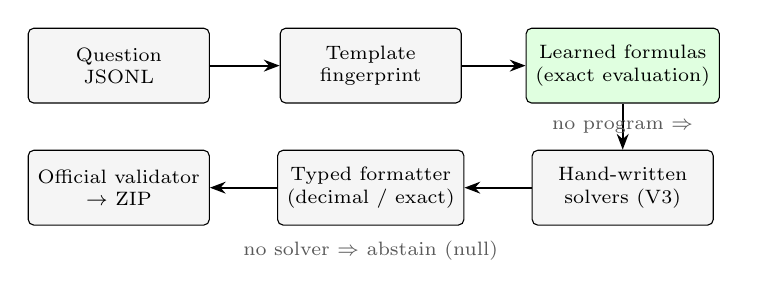
\begin{tikzpicture}[
  box/.style={draw,rounded corners=2pt,minimum width=2.3cm,minimum height=0.95cm,
              font=\scriptsize,align=center,fill=gray!8},
  learn/.style={box,fill=green!12},
  arr/.style={-{Stealth[length=2mm]},thick}]
  \node[box]   (q) at (0,0)    {Question\\ JSONL};
  \node[box]   (f) at (3.2,0)  {Template\\ fingerprint};
  \node[learn] (l) at (6.4,0)  {Learned formulas\\ (exact evaluation)};
  \node[box]   (h) at (6.4,-1.55) {Hand-written\\ solvers (V3)};
  \node[box]   (o) at (3.2,-1.55) {Typed formatter\\ (decimal / exact)};
  \node[box]   (v) at (0,-1.55) {Official validator\\ $\rightarrow$ ZIP};
  \draw[arr] (q)--(f); \draw[arr] (f)--(l); \draw[arr] (l)--(h);
  \draw[arr] (h)--(o); \draw[arr] (o)--(v);
  \node[font=\tiny,gray!60!black,right=2pt of l,yshift=-6pt,anchor=west,xshift=-1mm] {};
  \node[font=\tiny,gray!70!black] at (6.4,-0.78) {\scriptsize no program $\Rightarrow$};
  \node[font=\tiny,gray!70!black] at (3.2,-2.35) {\scriptsize no solver $\Rightarrow$ abstain (null)};
\end{tikzpicture}}
\caption{System overview. Learned formulas (green) are the main component; the
hand-written library is a fallback; the system abstains when neither applies.}
\label{fig_pipeline}
\end{figure}

\subsection{Fingerprints and number extraction}
The fingerprint is the question text with every number replaced by a placeholder,
paired with the tuple of slot identifiers. For a matching question we extract
all numeric tokens in order. (Some templates appear with more than one wording, so the 290 templates give rise to 340 distinct fingerprints in the training data.) Tokens may carry thousands separators, a percent
sign (converted to a fraction of one), or be fractions such as $p/q$. All values
are stored as exact rational numbers. A template is learnable only if every
labeled instance yields the same number $k\le 10$ of tokens; this excludes
templates whose wording contains a variable-length list.

\subsection{Search space}
Let $\ell_1,\dots,\ell_k$ be the extracted numbers and let $\mathcal{C}$ be a
fixed set of 13 constants (small integers, 12, 100, 360, 365, 1000, 52 and
$\tfrac12$). Expressions are defined by
\begin{equation}
\begin{gathered}
E ::= \ell_j \;\mid\; c \;\mid\; s_t \;\mid\; E \circ E,\\
\circ\in\{+,-,\times,\div,\max,\min,\wedge\},
\end{gathered}
\label{eq_grammar}
\end{equation}
where $c\in\mathcal{C}$, $s_t$ is the value of an earlier published step, and
$a\wedge b=a^{b}$ is allowed only for integer exponents with $|b|\le 60$. The
size of an expression is its number of leaves.

\subsection{Learning one template}
Algorithm~\ref{alg_learn} summarizes the procedure. Steps are learned in their
published order, and each verified step becomes a leaf for later steps and for
the final answer. This chaining is important: a final answer is usually a
simple function of the preceding steps, so it is found at size two or three even
when its expression in raw numbers would be much larger.

\begin{figure}[!t]
\centering
\fbox{\parbox{0.94\columnwidth}{\footnotesize
\textbf{Algorithm 1:} \textsc{LearnTemplate}\\[2pt]
\textbf{Input:} $m$ labeled instances of one template, each with numbers
$x_i$, step values $s_{i,t}$ and final value $y_i$.\\
1.\ \textbf{if} instances disagree on the token count $k$, or $k>10$:
abstain.\\
2.\ Leaves $\mathcal{L}\leftarrow\{\ell_1..\ell_k\}\cup\mathcal{C}$
(each a vector over the $m$ instances).\\
3.\ \textbf{for} each step $t$ in published order:\\
\hspace*{1.2em}$e_t\leftarrow\textsc{Search}(\mathcal{L},\,s_{\cdot,t},\,\text{exact})$;\\
\hspace*{1.2em}\textbf{if} $e_t$ verifies in exact arithmetic on all
instances: $\mathcal{L}\leftarrow\mathcal{L}\cup\{s_{\cdot,t}\}$.\\
4.\ $e_y\leftarrow\textsc{Search}(\mathcal{L},\,y,\,\text{round}(d))$; accept
only if exact verification passes.\\
5.\ \textbf{return} programs $(e_1,\dots,e_T,e_y)$; unsolved steps are
omitted.\\[2pt]
\textsc{Search}: enumerate sizes $1..3$; deduplicate candidates by their value
vector; return the first candidate that matches the target; for exact
targets, also test every pair (pool item $a$, pool item $b$) with
$a\circ b=\text{target}$ by a hash lookup.}}
\caption{Pseudo-code of the template learner.}
\label{alg_learn}
\end{figure}

\textbf{Value-signature pruning.} Two candidates that take the same values on
all $m$ instances are interchangeable for the purpose of search, so only the
first is kept. Signatures are the rounded value vectors, stored in a hash index.
Candidates are generated size by size with vectorized operators.

\textbf{Meet-in-the-middle.} For exact targets $t$ (published step values are
exact), instead of enumerating beyond size three we test, for every pool item
$a$ and each operator, whether the complementary vector ($t-a$, $a-t$, $t/a$ or
$a/t$) is itself in the pool. This detects expressions of up to six leaves at the
cost of a pool of size three, and it is how we recover the step formulas of four and five leaves.

\textbf{Rounding-aware matching.} A final answer is published rounded to $d$
decimal places, so a candidate $\hat y$ matches an instance when
\begin{equation}
|\hat y_i-y_i|\le \tfrac12\cdot 10^{-d}\quad\text{for all } i=1..m,
\label{eq_round}
\end{equation}
after which the candidate is re-evaluated in exact arithmetic and compared after
half-up rounding, so no floating-point match is accepted without verification.
Because the target is itself rounded, the meet-in-the-middle shortcut is not
applied to finals.

\textbf{Exact verification.} Search runs on double-precision vectors for speed.
Every accepted program is re-evaluated on every labeled instance with rational
numbers, and a program that disagrees anywhere is discarded. This establishes
agreement with the labeled instances under the scoring rules, with the same
rounding and canonicalization. It does not establish that the program is the
template's true formula: a program that coincides with the truth on every
labeled instance but differs on an unexercised corner is accepted, as the
zero-coupon error of Section~\ref{sub_failures} shows.

\subsection{Hand-written library}
The hand-written library contains exact solvers for 17 of the 290 templates:
five in accounting and financial reporting (balance sheets, cash-flow and income
statements), four in financial ratios (liquidity, leverage, efficiency and
profitability), two each in crypto finance (sentiment, whale detection), mergers
and acquisitions (due diligence), personal finance (budgeting, retirement
saving) and risk management (risk metrics, sensitivity analysis). Fourteen are
basic, two intermediate and one advanced. Each solver is guarded by the wording
of its template and was verified against the labeled instances.

\subsection{Implementation notes}
Several details affect reproducibility. Percent tokens are converted to
fractions of one and thousands separators are removed; negative numbers and
fractions $p/q$ are parsed exactly, but numbers written in words are not.
Search vectors are double-precision; candidate signatures are rounded to four
decimals, so two candidates that differ below that threshold are merged, which
can hide an alternative but never creates a false match because every accepted
program is re-checked exactly. Division by zero yields an invalid candidate that
is discarded, powers are allowed only for integer exponents of magnitude at most
60, and at most $4\times10^{5}$ new candidates are kept per operator and size
level, drawn with a fixed random seed so that runs are deterministic. Steps that
are not learned are skipped consistently when learning and when predicting, so
later expressions always refer to the same leaves. Finally, a program is applied
only when the new question yields exactly the same number of numeric tokens as
the labeled instances of its template.

\subsection{Prediction, formatting and combination}
At prediction time the program is evaluated on the extracted numbers of the new
question, step by step, with exact arithmetic. The result is rendered according
to its specification: half-up rounding to the stated number of places for
decimals, and the decimal-or-fraction rule of Section~III-B for exact values.
Steps with no learned program are omitted, and a question with no final program
receives a null final answer but still returns its solved steps. The
hand-written library of 17 verified templates takes precedence for the final
answer when it applies; its answers were exactly correct in every labeled case.

% =====================================================================
\section{Evaluation Protocol}
\label{sec_protocol}
\textbf{Held-out design.} The development split contains one labeled instance of
each of the 290 templates, none of which is used for learning. We learn from the
2{,}900 training instances (about ten per template) and score the 290 dev
instances with the organizers' scorer. This estimates how well a learned formula
generalizes to \emph{new instances of known templates}. It cannot estimate
performance on unseen templates, which the dev split does not contain.

\textbf{Metrics.} We report the number of correct final answers, the micro
final-answer score (correct divided by 290), the number of matched steps and the
micro trace score (matched divided by the 518 published slots). For a system that
abstains on $Q\setminus A$, with $C\subseteq A$ the exactly correct answers,
\begin{equation}
\text{precision}=\frac{|C|}{|A|},\qquad
\text{score}=\frac{|C|}{|Q|}=\frac{|A|}{|Q|}\cdot\text{precision}.
\label{eq_score}
\end{equation}
The scorer also reports two aggregates over the seen templates, which we list
alongside the micro scores.

\textbf{Systems.} (i)~\emph{Hand-written}: the 17-template library only.
(ii)~\emph{Learned}: the formula learner only. (iii)~\emph{Combined}: the
pipeline of Fig.~\ref{fig_pipeline}.

\textbf{Compute.} Learning all templates from the training data takes about two
minutes on a single CPU core, and prediction is instantaneous.

% =====================================================================
\section{Results}
\label{sec_results}
\subsection{Main comparison}
Table~\ref{tab_main} gives the official scores on held-out dev instances. The
learned solver answers 192 questions and 191 of them are exactly correct, a
precision of 99.5\% and a final-answer score of 0.659, more than ten times the
hand-written library. It also produces reasoning steps, matching 332 of 518
slots (0.641), whereas the hand-written library returns none. Adding the
hand-written library on top recovers three further answers (194 in total),
which shows that the two components are largely redundant on seen templates.
Wilson 95\% intervals for the learned solver are 97.1--99.9\% for precision,
60.2--71.1\% for the final-answer score and 59.9--68.1\% for the trace score, so
the differences between the systems are far outside the sampling noise.

\begin{table}[!t]
\renewcommand{\arraystretch}{1.25}
\caption{Held-Out Dev Results with the Organizers' Scorer (290 Questions,
518 Step Slots)}
\label{tab_main}
\centering
\footnotesize
\setlength{\tabcolsep}{3pt}
\begin{tabular}{@{}lrrrrrr@{}}
\hline
\bfseries System & \bfseries Final & \bfseries FAC & \bfseries Seen & \bfseries Steps & \bfseries Trace & \bfseries Seen\\
 & \bfseries correct & \bfseries micro & \bfseries FAC & \bfseries matched & \bfseries micro & \bfseries trace\\
\hline\hline
Hand-written & 17 & 0.059 & 0.060 & 0 & 0.000 & 0.000\\
Learned & 191 & 0.659 & 0.659 & 332 & 0.641 & 0.727\\
Combined & 194 & 0.669 & 0.668 & 332 & 0.641 & 0.727\\
\hline
\end{tabular}
\end{table}

\subsection{By domain and difficulty}
Fig.~\ref{fig_heldout_domain} shows the held-out accuracy by domain. Crypto
finance (94\%), personal finance (88\%), financial ratios (85\%) and accounting
and reporting (85\%) are best covered, while finance regulation (28\%),
investment analysis (32\%) and sustainable finance (36\%) are hardest. The
hand-written library is nearly absent in all but two domains.
Table~\ref{tab_difficulty} shows a monotone decline with difficulty: 81.0\% of
basic questions are correct, against 64.7\% of intermediate and 37.9\% of
advanced ones. Step matching follows the same trend (81\%, 67\% and 45\% of
slots). In finance regulation and sustainable finance the learner recovers a few
final formulas but almost none of the step formulas (7 of 42 and 9 of 51 slots),
which suggests that these domains use rule-based logic outside our arithmetic
grammar; we have not analyzed them further.

\begin{figure}[!t]
\centering
\includegraphics[width=\columnwidth]{figures/fig_heldout_domain.pdf}
\caption{Held-out dev accuracy by domain for learned formulas and for the
hand-written library (percentage of the questions of each domain answered
exactly right).}
\label{fig_heldout_domain}
\end{figure}

\begin{table}[!t]
\renewcommand{\arraystretch}{1.25}
\caption{Held-Out Dev Results by Difficulty}
\label{tab_difficulty}
\centering
\begin{tabular}{lrrrrr}
\hline
\bfseries Difficulty & \bfseries $n$ & \bfseries Hand & \bfseries Learned & \bfseries Learned (\%) & \bfseries Steps\\
\hline\hline
Basic & 116 & 14 & 94 & 81.0 & 102/126\\
Intermediate & 116 & 2 & 75 & 64.7 & 161/240\\
Advanced & 58 & 1 & 22 & 37.9 & 69/152\\
\hline
\end{tabular}
\end{table}

\subsection{Effect of checkpoint chaining}
\label{sub_chain}
Chaining, in which a learned step becomes a leaf for later expressions, is the
design choice we expected to matter most, and we isolate it with two ablations
that hold the search budget fixed: the maximum expression size stays at three,
the candidate caps are unchanged, and only the set of leaves differs.
\emph{No final chaining} forbids the final-answer expression from referencing
learned steps, while steps may still chain. \emph{No chaining} also forbids a
step from referencing earlier steps. Table~\ref{tab_chain} and
Fig.~\ref{fig_chaining} give the held-out results by the number of published
steps.

Final-answer accuracy collapses without chaining: 191 correct answers fall to
75 ($-61\%$), and precision is unchanged (75 of 75), so chaining adds coverage
rather than errors. Questions with no steps form a natural control and are
identical in all three settings (31 of 32). The effect grows with the number of
steps: one-step questions fall from 64 to 38 correct, two-step questions from 73
to 4, and three-step questions from 23 to 2. With the budget fixed, a final
answer written in raw numbers needs more than three leaves, whereas written over
checkpoints it is typically a single binary operation. Chaining matters much
less for the steps themselves: allowing none removes 23 of 332 matched slots
(7\%), all in two- and three-step questions (6 and 17 slots). Learning time rises
from 114\,s to 145\,s and 168\,s without chaining because the raw-number pools
are larger. Even with chaining, accuracy falls as steps accumulate (97\%, 93\%,
62\% and 32\% for zero to three steps) because one unlearned step makes the final
answer unreachable, and step matching falls from 93\% of one-step slots to 48\%
of three-step slots. The comparison is conditional on the size budget: a deeper
search could recover some of the lost answers at a higher cost, which we did not
test.

\begin{table}[!t]
\renewcommand{\arraystretch}{1.25}
\caption{Checkpoint-Chaining Ablation on Held-Out Dev, by Number of Published
Steps (Search Budget Fixed)}
\label{tab_chain}
\centering
\footnotesize
\setlength{\tabcolsep}{3pt}
\begin{tabular}{@{}lrrrrrr@{}}
\hline
 & & \multicolumn{3}{c}{\bfseries Correct final answers} & \multicolumn{2}{c}{\bfseries Slots matched}\\
\bfseries Steps & \bfseries $n$ & \bfseries Full & \bfseries No final & \bfseries None & \bfseries Full & \bfseries None\\
\hline\hline
0 & 32 & 31 & 31 & 31 & -- & --\\
1 & 69 & 64 & 38 & 38 & 64/69 & 64/69\\
2 & 118 & 73 & 4 & 4 & 166/236 & 160/236\\
3 & 71 & 23 & 2 & 2 & 102/213 & 85/213\\
\hline
All & 290 & 191 & 75 & 75 & 332/518 & 309/518\\
\hline
\end{tabular}
\end{table}

\begin{figure}[!t]
\centering
\includegraphics[width=\columnwidth]{figures/fig_chaining.pdf}
\caption{Share of held-out questions answered correctly with and without
reuse of learned steps in the final-answer expression, by the number of
published steps (search budget fixed).}
\label{fig_chaining}
\end{figure}

\subsection{How many examples are needed?}
Fig.~\ref{fig_learning_curve} varies the number of labeled instances per
template used for learning. With two examples the learner answers 197 questions
but only 154 are right (78.2\% precision), because many spurious formulas fit
two points. Precision rises to 86.6\% with three examples, 95.3\% with five,
98.4\% with seven and 99.5\% with ten, while the number of answered questions
barely changes. In other words, additional examples buy \emph{precision}, not
coverage. This is the practical reason that the organizers' ten instances per
template suffice, and it argues against learning from fewer examples without an
independent check.

\begin{figure}[!t]
\centering
\includegraphics[width=\columnwidth]{figures/fig_learning_curve.pdf}
\caption{Effect of the number of labeled instances per template on held-out
correct answers (left axis) and precision (right axis).}
\label{fig_learning_curve}
\end{figure}

\subsection{Ablations}
Table~\ref{tab_ablation} removes one component at a time. Restricting expressions to two leaves already solves 133 questions in
4.3\,s with no errors, which shows that most financial templates are shallow:
the typical final answer is a binary operation over numbers and earlier steps.
Removing the numeric constants costs 53 correct answers and 89 matched steps,
since conversions such as $\div 100$, $\times 12$ or $\div 365$ appear in many
formulas. Removing $\max$, $\min$ and powers costs 35 answers, so conditional
choices and compounding are not rare. The full system adds the remaining 58
answers on top of the size-two baseline at a cost of about 100\,s of search.

\begin{table}[!t]
\renewcommand{\arraystretch}{1.25}
\caption{Ablations on Held-Out Dev (Learned Solver Only)}
\label{tab_ablation}
\centering
\setlength{\tabcolsep}{4pt}
\begin{tabular}{lrrrrr}
\hline
\bfseries Configuration & \bfseries Answ. & \bfseries Corr. & \bfseries Prec. (\%) & \bfseries Steps & \bfseries Time (s)\\
\hline\hline
Full system & 192 & 191 & 99.5 & 332 & 107\\
No pow / max / min & 157 & 156 & 99.4 & 302 & 89\\
No constants & 139 & 138 & 99.3 & 243 & 10\\
Size $\leq 2$ & 133 & 133 & 100.0 & 280 & 4\\
\hline
\end{tabular}
\end{table}

\subsection{Scaling with the number of numbers}
Fig.~\ref{fig_scaling} relates learning success and cost to the number $k$ of
numeric tokens in a question. The share of fingerprints for which a final
formula is learned falls from 96\% at $k=2$ and 91\% at $k=3$ to 73\% at
$k=4$ and roughly 45--50\% for $k=5$ to 9, and reaches 20\% at $k=10$. Learning
time grows with $k$ but remains small: the mean is 0.02\,s at $k=2$ and about
1.5\,s at $k\ge 7$, the slowest template takes 3.8\,s, and the whole training
set takes about 127\,s on one core. Because the 10\% slowest templates account
for 64\% of the time, the cost is dominated by a few large pools. The practical
consequence is that the limit of the method is search depth, not compute: there
is ample time budget to search deeper before the cost becomes a problem. The
48 fingerprints with $k>10$ are not attempted at all.

\begin{figure}[!t]
\centering
\includegraphics[width=\columnwidth]{figures/fig_scaling.pdf}
\caption{Learning success (top) and mean learning time (bottom) by the number
of numeric tokens $k$ in the question; $n$ is the number of training
fingerprints in each group.}
\label{fig_scaling}
\end{figure}

\subsection{What the learned programs look like}
Of the 194 final-answer programs, one has one leaf, 155 have two and 38 have
three; the 364 step programs range from one to five leaves (16, 216, 107, 23
and 2 programs of one to five leaves). Multiplication (233 uses) and division (180)
dominate, followed by subtraction (152) and addition (125); $\min$ (27),
$\max$ (15) and powers (6) are rarer but necessary for the harder templates.

\subsection{Case studies}
The recovered programs read like textbook definitions. Table~\ref{tab_cases}
lists five of them in the notation of Eq.~(\ref{eq_grammar}), where $n_j$ is
the $j$-th number in the question, $t_i$ the $i$-th published step and $y$
the final answer. For example, the acquisition template is solved as
consideration ($t_1$) minus the fair value of net identifiable assets ($t_3$),
that is, goodwill; the inventory template divides 365 by the turnover ratio
$t_3$ to obtain days outstanding; and the impairment templates use $\min$ and
$\max$ to cap a reversal and to select the recoverable amount. Template names
in the table are our paraphrase of the question text.

\begin{table}[!t]
\renewcommand{\arraystretch}{1.3}
\caption{Examples of Learned Programs}
\label{tab_cases}
\centering
\footnotesize
\begin{tabular}{@{}p{0.31\columnwidth}p{0.62\columnwidth}@{}}
\hline
\bfseries Template (paraphrase) & \bfseries Learned program\\
\hline\hline
Acquisition goodwill & $t_1{=}n_1{+}n_2n_3$;\ $t_2{=}n_4{+}n_5{+}n_6$;\ $t_3{=}t_2{-}(n_7{+}n_8)$;\ $y{=}t_1{-}t_3$\\
Current ratio after loan reclassification & $t_1{=}n_1/n_2$;\ $t_2{=}n_2{+}n_4$;\ $t_3{=}n_1/t_2$;\ $y{=}t_1{-}t_3$\\
Days inventory outstanding & $t_1{=}n_1{+}n_2{-}n_3$;\ $t_2{=}\tfrac12(n_1{+}n_3)$;\ $t_3{=}t_1/t_2$;\ $y{=}n_5/t_3$ ($n_5{=}365$)\\
Impairment reversal cap & $t_1{=}n_2{-}n_1$;\ $y{=}\min(n_3,t_1)$\\
Impairment loss & $t_1{=}n_1{-}n_2$;\ $t_2{=}\max(n_3,n_4)$;\ $y{=}t_1{-}\min(t_1,t_2)$\\
\hline
\end{tabular}
\end{table}

\subsection{Failure taxonomy}
\label{sub_failures}
Fig.~\ref{fig_failures} classifies every held-out dev question. Of the 290, 191
are correct and one is wrong. The rest are abstentions: 44 where no formula of
size three was found, 34 whose text contains more than ten numbers, and 20 whose
answer is an enumerated choice, which the learner does not support. Among the 44 questions with no final formula, 32 have at least one learned
step and 10 have \emph{all} their steps learned, so a deeper or rounding-aware
final search would convert a number of near misses. The single
error is instructive: for a bond with a zero coupon rate, the learner returned
1026.81 for a gold value of 1010.00. In the ten training instances of that
template, a zero coupon rate occurred only together with zero elapsed days, so
the learner found a formula that depends on the elapsed days and coincides with
the truth on all of them. The held-out question probes the corner that the
training data never covered (a zero coupon with non-zero elapsed days). The
cause is therefore an under-determined training set, not an ambiguity between
equally simple formulas, as the next experiment shows.

\subsection{Example failures}
Three held-out questions illustrate the failure categories. Excerpts are
abridged.

\emph{Enumerated answer.} ``Direct ownership percent is 24.999. Indirect
ownership percent is 0. The scenario control flag is false. The ownership
threshold percent is 25. \dots\ Enhanced review is true when total ownership is
at least the threshold or the control flag is true.'' The answer is a Boolean
that follows from a comparison and a disjunction, so it is a classification of
computed quantities rather than a number. Our learner can compute the two
quantities but has no way to emit the choice.

\emph{Long numeric list.} ``A company has market-value common equity E of
106.24 USD million, debt A value DA of 34.76 \dots\ Let
rm=100*((1+rn/100)/(1+pi/100)-1), ke=rf+beta*(rm-rf), D=DA+DB,
kd=(DA*ka+DB*kb)/D, V=E+D, wE=E/V, wD=D/V, and real WACC=\dots'' The question
contains 18 numbers, so it exceeds our limit of ten. It also states every
formula explicitly, which makes it the clearest case for parsing the stated
calculation instead of searching for it.

\emph{No formula found.} ``An asset costs 100000 USD, has zero residual value,
and a useful life of 9 years. It receives 9 months of straight-line
depreciation in its acquisition year, then 4 complete depreciation years before
disposal. \dots\ Compute signed disposal gain or loss = sale price minus carrying
amount.'' Five numbers are involved, but the carrying amount needs a nested
composition (annual depreciation, then partial-year and full-year charges, then
their sum) that exceeds size three in raw numbers; the published steps lessen
this, but not enough for the search to close the gap.

\subsection{Ambiguity-aware abstention: a negative result}
A natural safeguard is to keep \emph{all} expressions of minimal size that fit
the examples and to abstain when they disagree on a new question. We implemented
it for final answers. On the training data, 128 of the 194 templates with a
learned final formula have more than one equally small candidate, so ambiguity
is common. Yet on the held-out dev questions the candidates always agree: the
system answers 192 questions and 191 are correct both with and without the
check. The check does not remove the single error, because the competing
candidates there agree with each other and are wrong together. Corner cases
that the labeled instances never exercise need a different remedy, for example
instance selection or a prior from the question text (Section~\ref{sec_future}).

\begin{figure}[!t]
\centering
\includegraphics[width=\columnwidth]{figures/fig_failures.pdf}
\caption{Outcome of every held-out dev question.}
\label{fig_failures}
\end{figure}

\subsection{Final test results}
We trained on the training and development data together (3{,}190 labeled
instances) and applied the system to the test set. It answers 406 of 928
questions (43.8\%): 55 from the hand-written library and 351 from learned
formulas, all of the latter in questions whose template is known. It also
returns 650 of the 1{,}492 published step values (43.6\%). These counts
measure coverage (non-null final answers and populated steps), not correctness,
which the official scores below report. Fig.~\ref{fig_test} shows where the remaining questions fall: 183 use a known
template that the system does not solve, and 339 use an unseen template
(Table~\ref{tab_test_causes}).

The organizers published the final test results on 28 October 2026
\cite{finreason2026results}. Our last accepted submission was scored with 377 of
928 final answers correct, a combined final-answer score (FAC) of 0.3364, a
hidden-stratum FAC of 0.0555 and a combined checkpoint (reasoning-step) score of
0.3450, which places the team 27th of 27 teams (Table~\ref{tab_final},
Fig.~\ref{fig_final}). The scored file is the 406-answer submission analyzed in
this paper: our earlier accepted files contained at most 60 non-null answers each
and could not have produced 377 correct ones, and the organizers score each team's
last accepted valid submission before the deadline. The combined scores weight a seen stratum (templates with
released examples) and a hidden stratum (templates without) equally, so the
seen-stratum FAC is implied to be $2\times0.3364-0.0555\approx0.617$. Three
observations follow.

\emph{The held-out protocol was well calibrated for seen templates.} The implied
seen-stratum score of 0.617 lies inside the 95\% interval of our held-out dev
estimate (60.2--71.1\%, point estimate 65.9\%) and is slightly lower, as
expected for a harder test mix.

\emph{The hidden stratum is out of reach for a template-level learner.} Its score
of 0.055 corresponds to roughly 20 of about 350 hidden questions. This is in
line with the 21 questions that the hand-written library answered in unseen
wording, which would mean that nearly all of those answers were right and that
the learner contributed nothing there, as designed.

\emph{Precision was lower than on held-out data.} Of the 406 questions answered,
377 were correct (92.9\%), against 99.5\% on held-out dev questions. If about 20
of the 21 hidden-stratum answers were right, then about 27 of the roughly 385
seen-stratum answers were wrong. We cannot locate these errors because test
answers are private, but the likeliest cause is the one found in
Section~\ref{sub_failures}: test instances contain parameter corners that the 11
labeled instances of a template never exercised, and one held-out instance per
template underestimates how often this happens. The implied figures here assume
the stated equal weighting of the two strata and are approximate.

The gap to the leading teams therefore has two parts. On the seen stratum, the
leaders are implied to reach about 0.998 against our 0.617, because our learner
solved only about two thirds of the known templates; on the hidden stratum they
reach 1.000 against our 0.055. Even the team ranked 26th is implied to score
about 0.977 on the seen stratum, so full coverage of the known templates was
within reach of a template-level method.

\begin{table}[!t]
\renewcommand{\arraystretch}{1.25}
\caption{Final Test Results (Frozen Scorer 2.0.0, 27 Teams, 928 Questions)}
\label{tab_final}
\centering
\footnotesize
\setlength{\tabcolsep}{3pt}
\begin{tabular}{@{}lccccr@{}}
\hline
\bfseries Entry & \bfseries Comb. & \bfseries Hidden & \bfseries Comb. & \bfseries Seen & \bfseries Correct\\
 & \bfseries FAC & \bfseries FAC & \bfseries ckpt. & \bfseries FAC$^{*}$ & \bfseries /928\\
\hline\hline
Rank 1 & 0.9992 & 1.0000 & 0.9996 & 0.9983 & 927\\
Rank 14 (median) & 0.9923 & 0.9897 & 0.9532 & 0.9950 & 921\\
Rank 26 & 0.4883 & 0.0000 & 0.4899 & 0.9767 & 566\\
This work (rank 27) & 0.3364 & 0.0555 & 0.3450 & 0.6173 & 377\\
\hline
\multicolumn{6}{@{}l}{\scriptsize $^{*}$Implied: 2 $\times$ combined FAC $-$ hidden FAC.}\\
\end{tabular}
\end{table}

\begin{figure}[!t]
\centering
\includegraphics[width=\columnwidth]{figures/fig_final_results.pdf}
\caption{Final test results of the 27 teams: implied seen-stratum score versus
hidden-stratum score. Most teams cluster near the top right; this work scores
well below the others on both strata.}
\label{fig_final}
\end{figure}

\begin{figure}[!t]
\centering
\includegraphics[width=\columnwidth]{figures/fig_test_composition.pdf}
\caption{Coverage of the system on the 928 test questions (non-null final
answers, not correctness), by source and by whether the template appears in the
labeled data.}
\label{fig_test}
\end{figure}

\begin{table}[!t]
\renewcommand{\arraystretch}{1.25}
\caption{Test-Set Coverage by Cause (Non-Null Final Answers, Not Correctness)}
\label{tab_test_causes}
\centering
\begin{tabular}{lrr}
\hline
\bfseries Outcome & \bfseries Questions & \bfseries Share (\%)\\
\hline\hline
Answered: learned formula & 351 & 37.8\\
Answered: hand-written library & 55 & 5.9\\
Not answered: known, no formula & 84 & 9.1\\
Not answered: known, over 10 numbers & 61 & 6.6\\
Not answered: known, enum answer & 38 & 4.1\\
Not answered: unseen, numeric & 256 & 27.6\\
Not answered: unseen, enum answer & 83 & 8.9\\
\hline
Total & 928 & 100.0\\
\hline
\end{tabular}
\end{table}

% =====================================================================
\section{Discussion}
\textbf{What we learned.}
(1) \emph{Most templates are shallow.} Two-leaf expressions over numbers and
earlier steps solve 133 held-out questions in about four seconds. Heavy
machinery is not needed for the first two thirds of the benchmark.
(2) \emph{Steps are the key.} The published intermediate steps turn a deep
search into a sequence of shallow ones. At a fixed search budget, forbidding the
final answer from using learned steps cuts correct answers from 191 to 75, and
to 4 of 118 for two-step questions (Section~\ref{sub_chain}).
(3) \emph{Examples buy precision.} The learner's coverage is nearly flat in the
number of examples, but its precision climbs from 78\% to 99.5\%, so the number
of labeled instances should be set by the precision one is willing to accept.
(4) \emph{Abstention is cheap and valuable.} A wrong answer scores the same as a
silence, but a wrong answer on a hidden test set cannot be detected; the
exactly verified, abstaining design gave 99.5\% precision on held-out dev
questions and 92.9\% on the answered test questions.
(5) \emph{The hand-written library was largely redundant.} Months of per-template
engineering are subsumed by two minutes of learning; the hand-written
solvers add only three answers.
(6) \emph{Coverage decides the ranking.} The final results show that the seen
stratum is nearly saturated by competitors and the hidden stratum is exactly
solvable by the ten best teams. Our learner recovers formulas for about two
thirds of the known templates, and that incomplete coverage, not precision, was
the main limit on the seen stratum.

\textbf{Practical lessons.} Two engineering choices paid off. First,
gating every upload on the official validator caught a formatting error that
would have invalidated most of our learned output: on the first test build the
validator rejected 207 rows because exact values that terminate had been written
as fractions; after the fix, all 468 rows with content were accepted. Second,
using the organizers' own scorer for held-out evaluation removed any doubt about
rounding and canonicalization conventions, which for exact-match scoring are as
decisive as the formulas themselves.

\textbf{Implications for benchmark design.} The development leaderboard has
99.7\% known templates, so a method that has learned the templates saturates it
while saying nothing about reasoning on new problems. The organizers' scorer
reports separate \emph{seen} and \emph{hidden} aggregates, and the final results
bear this out: the best ten teams are separated by less than 0.004 in combined
FAC and all reach at least 0.998 on the hidden stratum, whereas the bottom of
the table is separated by the hidden stratum and by template coverage. We
encourage participants to report both aggregates.

\textbf{Threats to validity.} Exact verification establishes agreement with the
labeled examples, not correctness on new instances; the zero-coupon error and
the drop in precision on test illustrate the gap. The held-out protocol measures
generalization to new instances of seen templates only. The final results show that it was well
calibrated there (implied seen-stratum score 0.617 against a held-out estimate
of 0.659), but it says nothing about hidden templates. Precision fell from 99.5\%
on held-out questions to 92.9\% on the answered test questions, so one held-out
instance per template underestimates the rate of corner-case errors. The
implied seen-stratum scores assume the organizers' equal weighting of the two
strata and are approximate. The template fingerprint is a surface heuristic and
may over- or under-count new templates; our estimate of 360 unseen test
questions is an upper bound and differs from the organizer-defined hidden
stratum (Section~\ref{sub_reuse}). The chaining ablation holds the expression
size fixed, so it measures the value of reuse at that budget, not in general. Finally, the leaderboard-development score of our
earlier hand-written-only submission (0.0529 final answer, 0.0 steps) reflects
an earlier system, not the one described here.

% =====================================================================
\section{How to Make It Better}
\label{sec_future}
The failure taxonomy converts directly into expected gains on seen templates,
in percentage points of the dev score:
\begin{enumerate}
  \item \textbf{Longer numeric lists (+11.7).} Thirty-four dev questions contain
        more than ten numbers, typically because they list several periods or
        positions. Aggregate leaves such as the sum, mean, minimum, maximum and
        prefix sums of the token list, together with a per-position leaf
        selector, would reduce them to the existing search.
  \item \textbf{Deeper formulas (+15.2).} Forty-four questions have no formula
        of size three. Type- and unit-aware search (never add a rate to an
        amount), operator-specific pruning, and a larger pool via beam search
        should reach sizes four and five. The step descriptions in the trace
        specification provide a vocabulary hint, for example that a step is a
        ``rate'' or an ``amount''.
  \item \textbf{Enumerated answers (+6.9).} Twenty questions ask for a choice.
        These are classification problems over computed quantities, such as
        comparing two plan costs, and can be learned as a comparison between
        two learned expressions with the choice labels read from the question.
  \item \textbf{Use the formula stated in the question.} Many question texts
        spell out the calculation: 103 of the 340 training fingerprints (30.3\%)
        contain an equals sign, as does 185 of the 928 test questions (19.9\%),
        and 28 of the 78 unsolved numeric dev questions. Parsing the stated
        formula would give a prior that rules out spurious fits such as the
        zero-coupon error, and would supply formulas to the deeper templates
        that the search cannot reach. The equals sign is only a crude proxy:
        only 16 of 360 unseen-template test questions contain one, yet the
        final results show that hidden templates can be solved exactly.
  \item \textbf{Unseen templates.} The ten best teams reach a hidden-stratum
        score of at least 0.998, so unseen templates are exactly solvable. One
        leading team's public repository reports 116 programs written for
        templates with no released instance~\cite{patodiya2026repo}, which
        matches roughly 350 hidden questions at three per template. We did not
        test how such programs are best obtained; the calculation stated in the
        question and the public FinChain generator~\cite{xie-etal-2026-finchain}
        are natural sources, and a language model that writes the program, with
        the arithmetic executed exactly as in program-aided
        models~\cite{gao2023pal} and the trace specification as an automatic
        check, is an alternative. Our verified-learner pipeline supplies the
        checking half and keeps the abstention behavior.
\end{enumerate}
Table~\ref{tab_headroom} converts the test-set causes into the number of
questions at stake for each improvement. Enumerated answers matter more on the
test set (121 questions, 13.0\%) than on dev (20 questions, 6.9\%), so item~3
deserves priority.

\begin{table}[!t]
\renewcommand{\arraystretch}{1.25}
\caption{Test Questions at Stake per Improvement}
\label{tab_headroom}
\centering
\begin{tabular}{lrr}
\hline
\bfseries Improvement & \bfseries Questions & \bfseries Share (\%)\\
\hline\hline
1. Longer numeric lists & 61 & 6.6\\
2. Deeper formulas & 84 & 9.1\\
3. Enumerated answers & 121 & 13.0\\
5. Unseen numeric templates & 256 & 27.6\\
\hline
\end{tabular}
\end{table}

Closing items 1--3 would, in principle, bring held-out dev accuracy from 0.659 to
1.0 and, on the test set, add up to 266 answered questions (28.7\%).

Fig.~\ref{fig_potential} shows the cumulative effect if each of these
improvements fully succeeded. These are upper bounds, not forecasts: the
largest step, unseen numeric templates, is also the hardest, and the earlier
steps are unlikely to be perfect. The figure is useful mainly for ordering the
work: items 1--3 together can add at most 266 questions (28.7\%) at modest
engineering cost, while the unseen templates require programs that must be
derived for each new template, which the final results show is feasible.

\begin{figure}[!t]
\centering
\includegraphics[width=\columnwidth]{figures/fig_potential.pdf}
\caption{Upper bounds on answered test questions as each improvement is added
cumulatively, starting from the current system (406 of 928).}
\label{fig_potential}
\end{figure}



% =====================================================================
\section{Conclusion}
Treating a templated benchmark as a programming-by-example problem was far more
productive than hand-writing solvers. A small formula learner with exact
verification and abstention recovers formulas for most known templates, answers
65.9\% of held-out dev questions with 99.5\% precision, matches 64.1\% of the
published reasoning steps, and raised test coverage from 55 to 406 answered
questions. In the official final results this gave a combined final-answer score
of 0.336 (rank 27 of 27): the seen-stratum score of about 0.62 matched our
held-out estimate, but incomplete coverage of known templates and the hidden
stratum, which a template-level learner cannot reach, explain the gap to the
leading teams. The remaining errors are well understood: coverage of known
templates (long numeric lists, deeper formulas, enumerated choices) and unseen
templates. We hope the ablations, the learning curve and the failure taxonomy
help other participants decide where to invest effort.

\section*{Acknowledgment}
We thank the FinReason Cup organizers for the public data, schemas, validator and
scorer.

\bibliographystyle{IEEEtran}
\bibliography{refs}

% =====================================================================
\appendices
\section{Search Space and Data Files}
\textbf{Constants.} The constant set is $\{1,2,3,4,5,10,12,100,365,360,1000,
\tfrac12,52\}$. Percent tokens in the text are converted to fractions of one.
\textbf{Operators.} $+$, $-$, $\times$, $\div$, $\max$, $\min$ and integer powers.
\textbf{Limits.} Maximum token count 10; maximum expression size 3 for
enumeration, up to 6 for exact targets through meet-in-the-middle; at most
$4\times10^{5}$ new candidates per operator and size level.

\section{Reproducibility}
All figures are produced by one script from CSV files that accompany the paper
(split-level coverage, answer types, per-template learning statistics,
held-out results by domain, difficulty and number of steps, the learning curve,
ablations, the chaining ablation, the failure taxonomy and the published final
test scores). The learner, the
evaluation scripts and the submission builder are included with the paper's
data. A submission is built by merging prediction files, keeping only rows that
pass the organizers' record validator, and then running the validate, package
and validate-zip commands of the public toolkit. The held-out numbers in
Table~\ref{tab_main} are obtained with the toolkit's development scorer.

\end{document}
